\documentclass[aspectratio=169]{beamer}

% --- Tema ---
\usetheme{Madrid}
\usecolortheme{default}

% --- Pacotes ---
\usepackage[utf8]{inputenc}
\usepackage[T1]{fontenc}
\usepackage[brazilian]{babel}
\usepackage{amsmath}
\usepackage{amssymb}
\usepackage{graphicx}
\usepackage{booktabs}
\usepackage{array}
\usepackage{algorithmicx}
\usepackage{algpseudocode}

% --- Cores institucionais ---
\definecolor{ufmgred}{RGB}{200,16,46}
\setbeamercolor{structure}{fg=ufmgred}
\setbeamercolor{title}{fg=white,bg=ufmgred}
\setbeamercolor{frametitle}{fg=white,bg=ufmgred}
\setbeamercolor{block title}{fg=white,bg=ufmgred}
\setbeamercolor{block body}{fg=black,bg=ufmgred!8}
\setbeamercolor{exampleblock title}{fg=white,bg=blue!65!black}
\setbeamercolor{exampleblock body}{fg=black,bg=blue!6}

% --- Metadados ---
\title[TP1 -- Cassotis]{Otimização Mono-objetivo de Pilhas de Minério}
\subtitle{Entrega 1 -- Case Cassotis}
\author[Grupo 1]{%
Felipe Augusto Cruz Sousa \and Gustavo Madureira Tavares de Melo \and
Henry Diniz Sepini Rodrigues Amaral \and Lucas Rodrigues Prosperi Ayala \and
Luisa Marques Laboissiere \and Thales Gregory Vasconcelos Santos}
\institute[UFMG]{Universidade Federal de Minas Gerais -- Escola de Engenharia}
\date{Setembro de 2026}
\titlegraphic{
\includegraphics[width=0.18\textwidth]{image.png}}

\begin{document}

% 1. Título
\begin{frame}
    \titlepage
\end{frame}

% 2. Agenda
\begin{frame}{Agenda}
    \tableofcontents
\end{frame}

% 3. Problema
\section{Problema e representação}
\begin{frame}{Problema e objetivos}
\begin{columns}[T]
    \begin{column}{0.52\textwidth}
        \begin{block}{Decisão}
            Definir a composição de dez pilhas que alimentam dois equipamentos
            de sinterização. Cada posição da solução representa um caminhão de
            2 kt.
        \end{block}

        \begin{exampleblock}{Restrições}
            Massa exata, compatibilidade minério--equipamento, disponibilidade
            mínima e máxima e limites de $SiO_2$ e $Al_2O_3$.
        \end{exampleblock}
    \end{column}

    \begin{column}{0.44\textwidth}
        \textbf{Três versões mono-objetivo}
        \begin{itemize}
            \item $f_1$: custo total de aquisição;
            \item $f_2$: desvio quadrático de $SiO_2$;
            \item $f_3$: desvio quadrático de $Al_2O_3$.
        \end{itemize}

        \vspace{0.4cm}
        O conjunto viável permanece o mesmo. Apenas a função objetivo muda.
    \end{column}
\end{columns}
\end{frame}

% 4. Representação e solução inicial
\begin{frame}{Representação e solução inicial}
\begin{columns}[T]
    \begin{column}{0.47\textwidth}
        \begin{block}{Representação}
            \[
                x = \{P_1,\ldots,P_{10}\}.
            \]
            Cada pilha é um vetor de minérios. Cada elemento corresponde a um
            caminhão de 2 kt.
        \end{block}

        A representação permite alterar ou trocar caminhões diretamente nas
        posições dos vetores.
    \end{column}

    \begin{column}{0.49\textwidth}
        \begin{exampleblock}{Heurística construtiva}
            \begin{enumerate}
                \item inserir as disponibilidades mínimas obrigatórias;
                \item completar as pilhas com o minério compatível de menor custo.
            \end{enumerate}
        \end{exampleblock}

        \textbf{Ponto inicial:} R\$ 60,4 milhões e 12 violações de qualidade.

        \vspace{0.3cm}
        As restrições estruturais são preservadas por construção. O GVNS trata
        as violações de qualidade.
    \end{column}
\end{columns}
\end{frame}

% 5. Pseudocódigo completo
\section{Metaheurística}
\begin{frame}{Pseudocódigo do GVNS completo}
\scriptsize
\begin{algorithmic}[1]
    \State $x^* \gets \textsc{SolucaoInicial}()$
    \State $sem\_melhora \gets 0$
    \For{$iter = 1$ até $\text{MAX\_ITER}$}
        \State $k \gets 1$
        \While{$k \leq K_{\max}$}
            \State $x' \gets \textsc{Shake}(x^*, k)$
            \State $x'' \gets \textsc{VND}(x', f)$
            \If{$\phi(x'') < \phi(x^*)$}
                \State $x^* \gets x''$; $k \gets 1$
            \Else
                \State $k \gets k + 1$
            \EndIf
        \EndWhile
        \State atualizar $sem\_melhora$
        \If{$sem\_melhora \geq \text{MAX\_SEM\_MELHORA}$}
            \State \textbf{pare}
        \EndIf
    \EndFor
    \State \Return $x^*$
\end{algorithmic}

\footnotesize
A função $\phi$ integra o objetivo e a penalização de qualidade. O retorno final
é validado estruturalmente e quanto aos limites químicos.
\end{frame}

% 6. Vizinhanças e busca
\begin{frame}{Vizinhanças, SHAKE e VND}
\begin{columns}[T]
    \begin{column}{0.48\textwidth}
        \begin{block}{$N_1$ e $N_2$}
            \begin{itemize}
                \item $N_1$: substitui um caminhão por outro minério compatível;
                \item $N_2$: troca caminhões entre pilhas com compatibilidade cruzada.
            \end{itemize}
        \end{block}

        \begin{alertblock}{$N_3$: decisão do grupo}
            Substitui dois caminhões da mesma pilha simultaneamente. O movimento
            permite ajustes combinados de qualidade que uma troca unitária pode
            não alcançar sem piorar o passo intermediário.
        \end{alertblock}
    \end{column}

    \begin{column}{0.48\textwidth}
        \begin{exampleblock}{SHAKE}
            Aplica $k$ movimentos aleatórios, com $k \in \{1,2,3\}$, preservando
            a viabilidade estrutural.
        \end{exampleblock}

        \begin{exampleblock}{VND}
            Percorre $N_1 \to N_2 \to N_3$ com \textit{First Improvement} e
            reinicia em $N_1$ quando encontra melhora.
        \end{exampleblock}

        As vizinhanças usam amostragem para controlar o custo computacional.
    \end{column}
\end{columns}
\end{frame}

% 7. Inviabilidade e parada
\begin{frame}{Inviabilidade, aceitação e parada}
\begin{columns}[T]
    \begin{column}{0.5\textwidth}
        \begin{block}{Tratamento de inviabilidade}
            Restrições estruturais são preservadas por construção ou rejeição.
            Violações de qualidade entram na função de \textit{fitness}:
            \[
                \phi(x) = f(x) + \lambda\,\mathrm{pen}(x).
            \]
            \[
                \lambda_{f_1}=10^{12},\qquad
                \lambda_{f_2}=\lambda_{f_3}=10^4.
            \]
        \end{block}
    \end{column}

    \begin{column}{0.46\textwidth}
        \begin{exampleblock}{Aceitação}
            O VND e o laço externo aceitam apenas soluções com \textit{fitness}
            estritamente menor.
        \end{exampleblock}

        \begin{alertblock}{Parada e limites internos}
            \begin{itemize}
                \item 200 iterações externas;
                \item parada após 60 iterações sem melhora;
                \item 20 vizinhos por busca local;
                \item no máximo 5 reinícios do VND.
            \end{itemize}
        \end{alertblock}
    \end{column}
\end{columns}
\end{frame}

% 8. Experimentos
\section{Experimentos e resultados}
\begin{frame}{Planejamento e resultados}
\small
Foram executadas cinco sementes para cada objetivo
($42$, $123$, $456$, $789$ e $1011$), totalizando 15 execuções.

\vspace{0.35cm}
\centering
\begin{tabular}{lrrrr}
\toprule
Objetivo & Mínimo & Média & Desvio-padrão & Máximo \\
\midrule
$f_1$ (R\$) & 60.300.000 & 60.512.000 & 159.123 & 60.680.000 \\
$f_2$       & 2,372757   & 2,373477   & 0,000543 & 2,373927 \\
$f_3$       & 1,436169   & 1,447180   & 0,007289 & 1,453254 \\
\bottomrule
\end{tabular}

\vspace{0.45cm}
\begin{block}{Resultado comum às 15 execuções}
Todas as soluções finais são estruturalmente válidas e atendem aos limites de
qualidade. $f_2$ apresentou a menor dispersão relativa; $f_3$ foi mais sensível
às sementes.
\end{block}
\end{frame}

% 9. Convergência e conclusão
\begin{frame}{Convergência e conclusão}
\centering
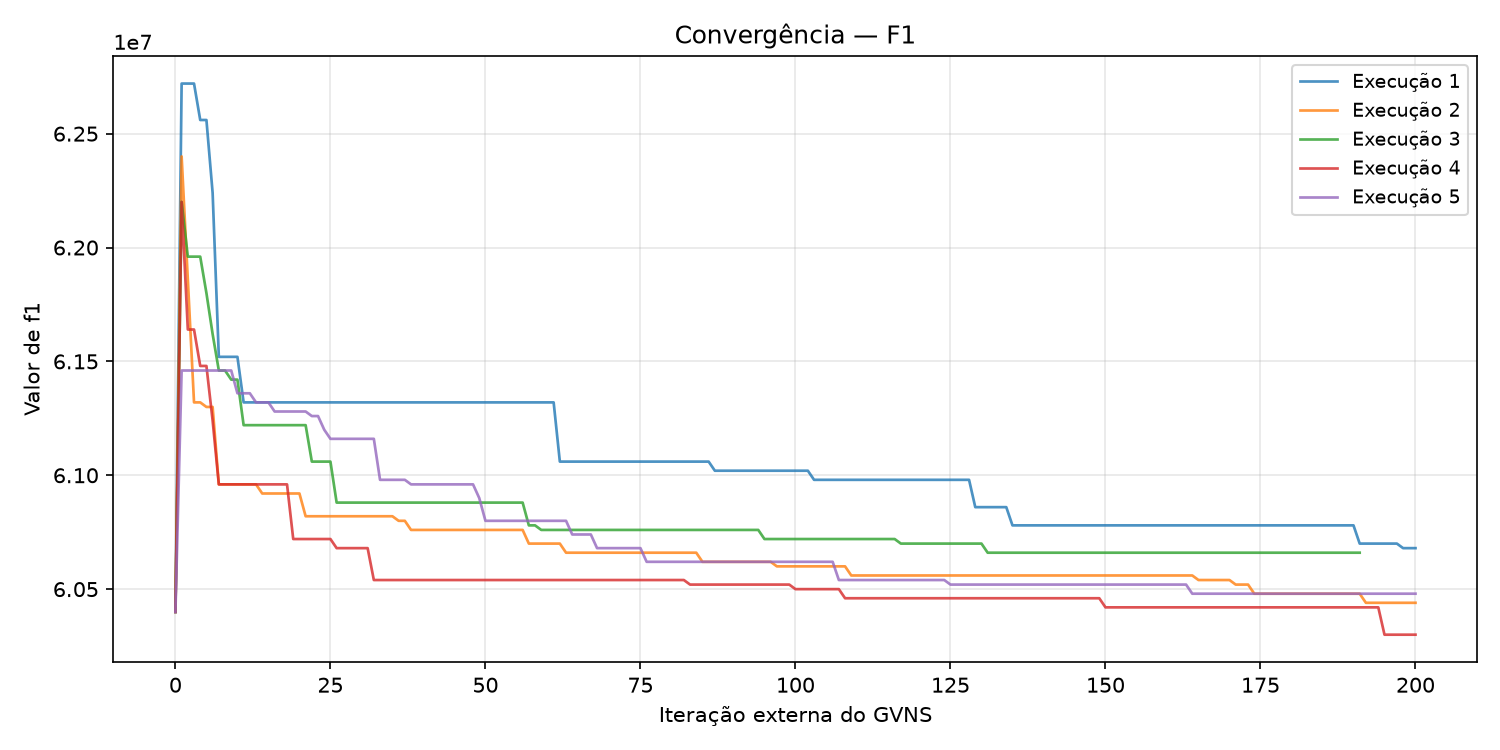
\includegraphics[width=0.32\textwidth]{convergencia_f1.png}\hfill
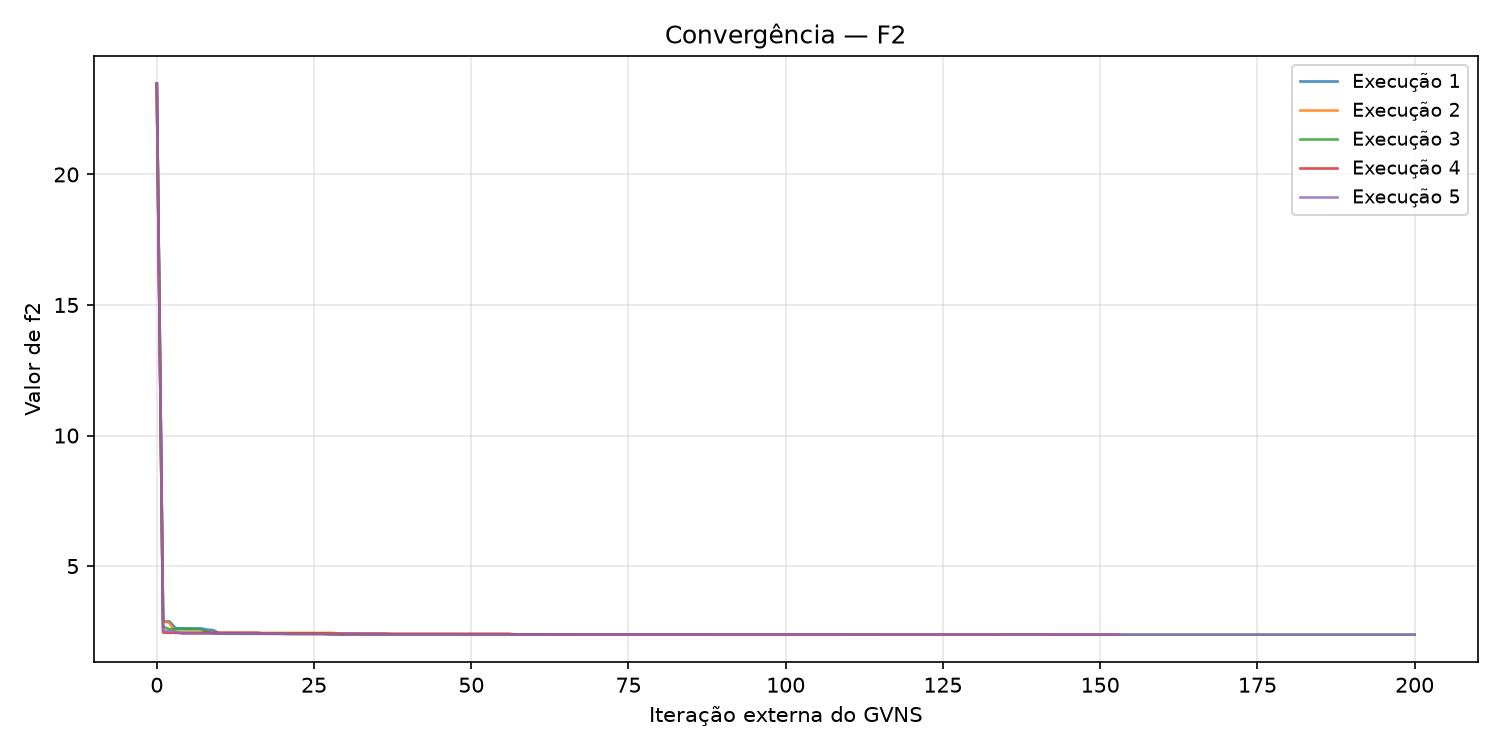
\includegraphics[width=0.32\textwidth]{convergencia_f2.png}\hfill
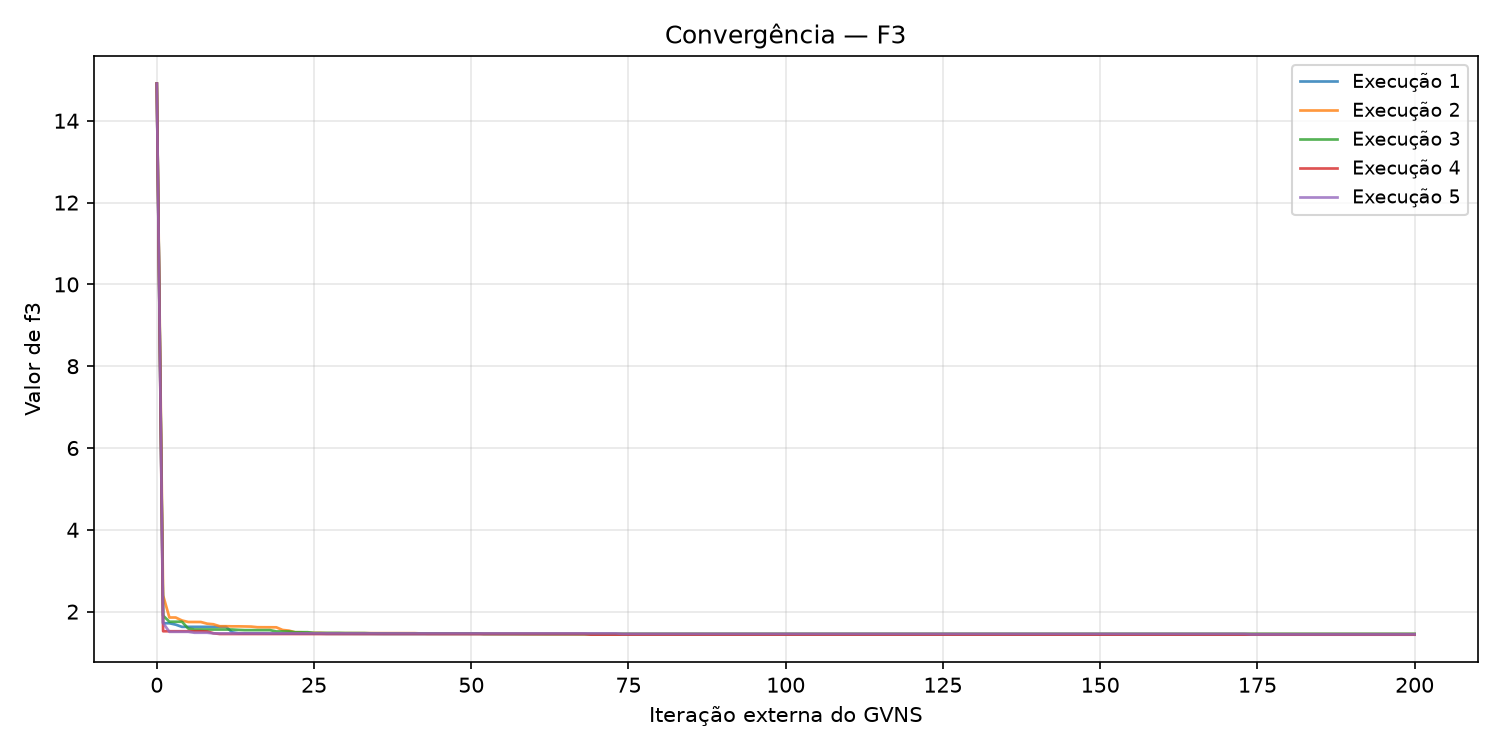
\includegraphics[width=0.32\textwidth]{convergencia_f3.png}

\vspace{0.3cm}
\begin{columns}[T]
    \begin{column}{0.62\textwidth}
        \begin{block}{Conclusões}
            \begin{itemize}
                \item o GVNS produziu soluções finais viáveis nas 15 execuções;
                \item os desvios de qualidade caíram cerca de 90\% em relação à solução inicial;
                \item N3, SHAKE, VND e penalização integraram diversificação e intensificação.
            \end{itemize}
        \end{block}
    \end{column}
    \begin{column}{0.34\textwidth}
        \begin{exampleblock}{Melhores valores}
            $f_1$: R\$ 60.300.000\\
            $f_2$: 2,372757\\
            $f_3$: 1,436169
        \end{exampleblock}
    \end{column}
\end{columns}
\end{frame}

\end{document}
